\documentclass{beamer}

\usepackage{graphicx} 			% Imagens
\usepackage{amsmath}			% Matemático
\usepackage{amsfonts}			% Fontes
\usepackage[utf8]{inputenc}		% Acentos
\usepackage{float}				% Incluir figura no minipage
\usepackage{multimedia}			% Vídeos

\title{Trabalhando com Apresentações}
\author[L. A. B.]{Lucas Arantes Berg}
\institute{Universidade Federal de Juiz de Fora}
\date{\today}
\usetheme{default}
\usecolortheme{orchid}

% Definindo cores
\setbeamercolor{cor1}{bg=blue!60!black,fg=white}
\setbeamercolor{cor2}{bg=white,fg=blue!60!black}

\begin{document}
	
	\begin{frame}
		\titlepage
	\end{frame}
	
	\begin{frame}
		\frametitle{Sumário}
		\tableofcontents[section,subsection]
		\section{Arritmias Cardíacas}
		\section{Sistema de Condução Cardíaco}
		\section{Potencial de Ação}
		\section{Testando vídeo}
	\end{frame}
	
	\begin{frame}
		\frametitle{Arritmias Cardíacas}
		\begin{center}
			\movie[externalviewer]{
\includegraphics[scale=0.2]{imagens/thumb-arritmia.png}}{videos/ventricular-arritmia.mp4}
		\end{center}
	\end{frame}
	
	\begin{frame}
		\frametitle{Sistema de Condução Cardíaco}
		\begin{center}
			\movie[externalviewer]{
\includegraphics[scale=0.2]{imagens/thumb-conducao.png}}{videos/sistema-conducao.mp4}
		\end{center}
	\end{frame}

	\begin{frame}
		\frametitle{Potencial de Ação}
		\begin{center}
			\movie[externalviewer]{
\includegraphics[scale=0.2]{imagens/thumb-pa.png}}{videos/potencial-acao.mp4}
		\end{center}
	\end{frame}
	
	\begin{frame}
		\frametitle{Simulação}
		\begin{center}
			\movie[scale,externalviewer]{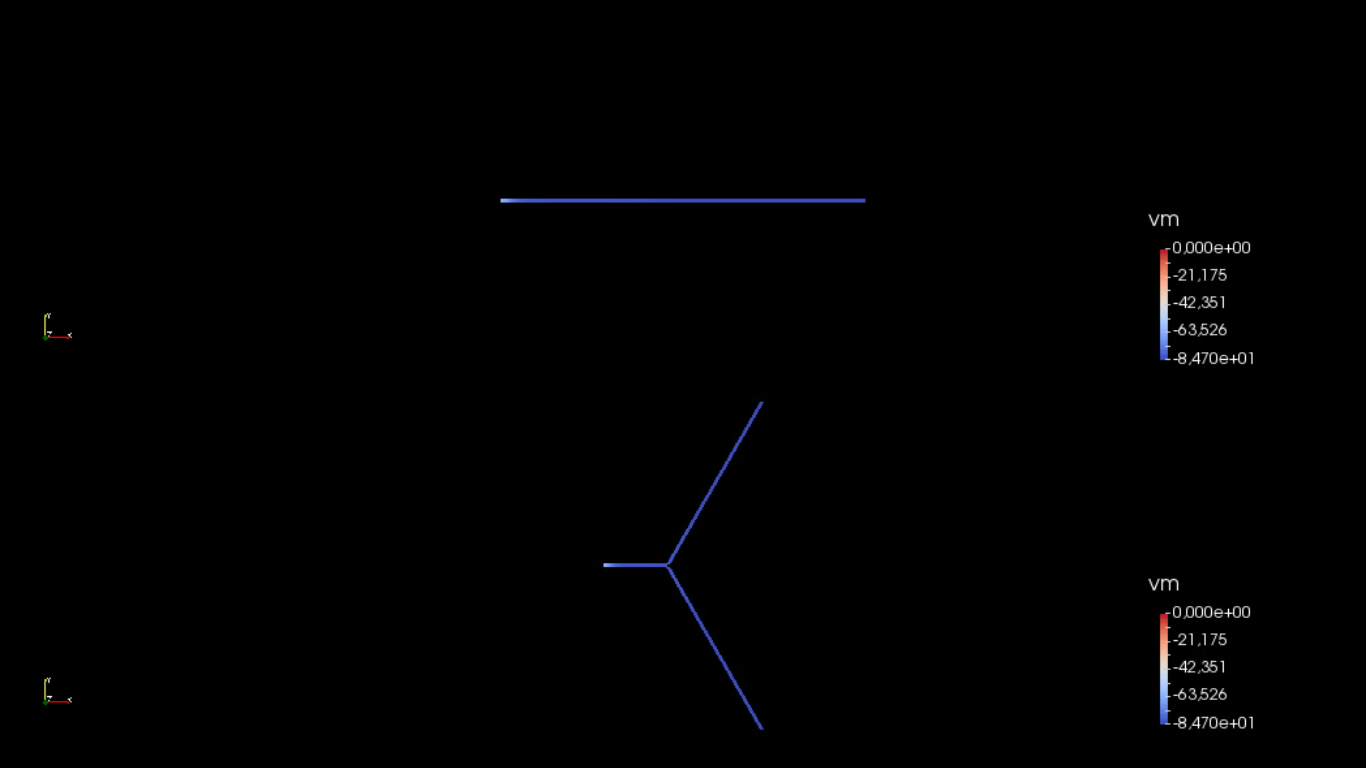
\includegraphics[scale=0.2]{imagens/thumb-simula.png}}{videos/simula.avi}
		\end{center}
	\end{frame}
\end{document}

